\documentclass[12pt,a4paper,oneside,openany]{article}
\usepackage[squaren]{SIunits}
%% LaTeX Preamble - Common packages
%\usepackage[german]{babel}
\usepackage{setspace}

\usepackage[T1]{fontenc}
\usepackage{cmap}
\usepackage[utf8]{inputenc} % Any characters can be typed directly from the keyboard, eg éçñ
\usepackage{textcomp} % provide lots of new symbols
\usepackage{graphicx}  % Add graphics capabilities
\usepackage{flafter}  % Don't place floats before their definition
%\usepackage{topcapt}   % Define \topcaption for placing captions above tables (not in gwTeX)
\usepackage[numbers]{natbib} % use author/date bibliographic citations
\usepackage{subfigure}
\usepackage{url}
%\usepackage{babelbib}
\usepackage{booktabs}

\usepackage{amsmath,amssymb}  % Better maths support & more symbols
\usepackage{bm}  % Define \bm{} to use bold math fonts
\usepackage{esint}
\usepackage{algorithm}
%\usepackage[noend]{algorithmic}
\usepackage{algorithmicx}
\usepackage{algpseudocode}

\usepackage[usenames,dvipsnames]{color} 

\usepackage[pdftex,bookmarks,colorlinks,breaklinks]{hyperref}  % PDF hyperlinks, with coloured links
%\definecolor{dullmagenta}{rgb}{0.4,0,0.4}   % #660066
%\definecolor{darkblue}{rgb}{0,0,0.4}
\hypersetup{linkcolor=red,citecolor=blue,filecolor=blue,urlcolor=blue} % coloured links
%\hypersetup{linkcolor=black,citecolor=black,filecolor=black,urlcolor=black} % black links, for print output

\usepackage[noabbrev,nameinlink,capitalize]{cleveref}

\usepackage{memhfixc}  % remove conflict between the memoir class & hyperref
% \usepackage[activate]{pdfcprot}  % Turn on margin kerning (not in gwTeX)
%\usepackage{pdfsync}  % enable tex source and pdf output syncronicity

\usepackage{listings}
\usepackage{nomencl}

%\usepackage{python}
\usepackage{tikz}
%\usetikzlibrary{arrows,decorations.pathmorphing,backgrounds,placments,fit}
\usetikzlibrary{calc,arrows,through,backgrounds,fit,shapes.geometric,shapes.misc,plotmarks}

\usepackage{anysize}
\marginsize{2cm}{2cm}{2cm}{2cm}

\onehalfspacing

\makenomenclature
\def\nomlabel#1{\textbf{#1}\hfil}

\newcommand{\Parameters}{\subsection*{Parameters}}
\newcommand{\ReturnValue}{\subsection*{Return Value}}
\newcommand{\Description}{\subsection*{Description}}
\newcommand{\ClassName}[1]{{\tt #1}}
\newcommand{\ReturnType}[1]{{\tt (#1)}}
%\newcommand{\Function}[1]{{\tt #1()}}
\newcommand{\Self}{{\tt self}}

\DeclareMathOperator{\erf}{erf}
%\DeclareMathOperator{\K}{K}
%\newcommand{\K}{\ensuremath{\mathrm{\large{K}}}}
\newcommand{\ud}{\ensuremath{\mathrm{d}}}
\newcommand{\ii}{\ensuremath{\mathrm{i}}}
\newcommand{\fclamp}{\ensuremath{\mathrm{clamp}}}
\newcommand{\vx}{\ensuremath{\boldsymbol{x}}}
\newcommand{\vv}{\ensuremath{\boldsymbol{v}}}
\newcommand{\va}{\ensuremath{\boldsymbol{a}}}
\newcommand{\vf}{\ensuremath{\boldsymbol{f}}}
\newcommand{\mM}{\ensuremath{\boldsymbol{M}}}
\newcommand{\mW}{\ensuremath{\boldsymbol{W}}}
\newcommand{\mJ}{\ensuremath{\boldsymbol{J}}}
\newcommand{\vq}{\ensuremath{\boldsymbol{q}}}
\newcommand{\vC}{\ensuremath{\boldsymbol{C}}}
\newcommand{\vQ}{\ensuremath{\boldsymbol{Q}}}
\newcommand{\vlambda}{\ensuremath{\boldsymbol{\lambda}}}
\newcommand{\vd}{\ensuremath{\boldsymbol{d}}}
\newcommand{\mI}{\ensuremath{\boldsymbol{I}}}
\newcommand{\vc}{\ensuremath{\boldsymbol{c}}}
\newcommand{\vr}{\ensuremath{\boldsymbol{r}}}
\newcommand{\vF}{\ensuremath{\boldsymbol{F}}}
\newcommand{\vtau}{\ensuremath{\boldsymbol{\tau}}}
\newcommand{\valpha}{\ensuremath{\boldsymbol{\alpha}}}

\newtheorem{mydef}{Definition}


\lstset{numbers=left,basicstyle=\footnotesize,numberstyle=\tiny,tabsize=4,breaklines=true}

\long\def\symbolfootnote[#1]#2{\begingroup%
\def\thefootnote{\fnsymbol{footnote}}\footnote[#1]{#2}\endgroup}


\begin{document}

\tableofcontents

\listoffigures

\section*{About}

This document contains notes about the \em Giddy Machinist \em project.

\section{Straight Skeleton Generation}


The straight skeleton is generated via a two-phase approach. At first, the so-called motorcycle graph is generated, then the actual straight skeleton. One algorithm is described in \cite{ski}.

There are single-phase and two-phase approaches. The two phase approach seems more robust for handling degenerate geometry, for example symmetric polygons, which are very common in practical usage. The two phase approach begins with the motorcycle tracing, which creates clear boundaries for non-convex polygons. 

Another advantage to the two phase approach is that principally, the time complexity of the 2nd phase is greatly reduced, as all events that need to be tracked are of time complexity $O(N+M)$, as there are only collapse events for each edge, as well as the wavefronts opposite of a motorcycle, that need to be tracked.

\subsection{The Motorcycle Graph}

For a simple polygon, motorcycles are only emitted by reflex\footnote{what exactly is a reflex vertex?} vertices. The motorcycles are angular bisector rays, and may crash into each other or the polygon edges as in the game \em Tron\em . A motorcycle trace is terminated when it reaches an edge or other motorcycle trace. A degenerate case, which must be handled for real-world geometry, is when two or more motorcycles collide at the same point, in which case a new motorcycle must be emitted.

\subsubsection{Events}

Three different events may happen during motorcycle tracing:
\begin{description}
\item[Edge Crash] The edge crash is the simplest event, and happens when a motorcycle hits a polygon edge. The edge is split (unless the hit is at an existing vertex), and a new vertex is inserted.
\item[Trace Crash] When a motorcycle hits the trace of another motorcycle, it is terminated, and a vertex is generated.
\item[Merge Crash] When two motorcycles reach the same point in space at the same time, they merge, and may emit one or two new motorcycles in new directions, depending on the crash geometry. This kind of crash can be ignored, and a trace crash can be used instead.
\end{description}


\subsubsection{Special Considerations}

The times for potential crashes do not change during tracing, but new motorcycles may be generated during merges.

Events are treated as simultaneous if they occur within some limit of location and time. As motorcycle events are point-like in nature, there is no danger of invalidating the graph.

\paragraph{Collinear Motorcycles}

A special degenerate case can occur when two motorcycles are collinear, but in opposite directions. In such a case, one of the motorcycles may be discarded. This commonly occurs in CAD data with aligned holes. Cases can occur when only one endpoint is shared, but the other is a trace crash site.

A special difficulty occurs when a motorcycle terminates near an outline vertex, and consequently slightly changes direction as it's nudged into the vertex.


\subsubsection{Tracing Algorithm}

The implementation is outlined in  \cref{alg:mc}. Large performance improvements could be made by eliminating redundant intersection queries.

\begin{algorithm}
\caption{Computation of motorcycle graph.}
\label{alg:mc}
\begin{algorithmic}
\Require{simple input polygon}
\For{each vertex}
	\State create motorcycle structure
\EndFor

\Repeat
	\For{each active motorcycle}
		\State record crash times with edges
		\State record crash times with active motorcycles
		\State record crash times with terminated motorcycles
	\EndFor
	\State sort crash events by time
	\State pick first crash
	\State assemble array off all crash events within merge threshold of location and time from first crash
	\State determine crash subtypes: wall, trace, merge
	\If {contains wall crash} 
		\State all traces terminate at crash site
		\If{not at vertex}
			\State split edge, insert new vertex
		\EndIf
	\ElsIf{contains trace crash}
		\State create new vertex, terminate crashed motorcycles
	\Else
		\State create new vertex, terminate involved motorcycles
		\If{non-convex sub-polygon remains}
			\State start new `escaped' motorcycle
		\EndIf
	\EndIf 

\Until{no more active motorcycles}
\end{algorithmic}
\end{algorithm}

\subsection{Wavefront Propagation}

After the motorcycle graph is generated, the wavefront propagation can be started. Each edge emits a wavefront, which can either collapse, or be split by a motorcycle.

\begin{algorithm}
\caption{Wavefront Initialization.}
\label{alg:wpi}
\begin{algorithmic}
\Require{simple input polygon}
\Require{motorcycle graph}
\For{each motorcycle}
	\State create motorcycle spoke and anti-spoke
\EndFor
\For{each vertex on outline}
	\State create spoke if vertex is convex, and no motorcycle spoke or anti-spoke exists
\EndFor
\For{each each spoke starting at $t=0$}
	\State create wavefront
	\State attach wavefront
\EndFor

\State generate emission events

\For{each wavefront}
	\State compute collapse time
	\State add collapse event to event queue
\EndFor

\For{each branch and merge vertex}
	\State add respective events to event queue
\EndFor

\For{each motorcycle spoke}
	\If{motorcycle starts on outline vertex}
		\State compute split event
	\EndIf
	\If{motorcycle ends on outline vertex}
		\For{each other motorcycle crashed into trace}
			\State compute reverse branch event
		\EndFor
		\If{motorcycle starts on merge vertex}
			\State compute reverse merge event
		\EndIf
	\EndIf
	\If{motorcycles ends and starts on outline}
		\State add earliest event to event queue
	\Else
		\State add split or reverse event to event queue, whichever exists
	\EndIf
\EndFor


\end{algorithmic}
\end{algorithm}

\subsubsection{Wavefront Events}

The following events may occur during wavefront propagation:
\begin{description}
\item[Wavefront Collapse] The collapse is the simplest event. A wavefront collapses into a vertex, which emits a new spoke bisecting the neighbouring wavefronts.
\item[Motorcycle Split] The split occurs along a motorcycle trace, when the motorcycle would hit the opposing face. As the wavefronts are already pre-split along the motorcycle trace, only minor topological changes need to happen.
\item[Motorcycle Branch] A branch occurs when a motorcycle trace reaches a point where another motorcycle will crash into it. The wavefront is split along the incoming motorcycle trace.
\item[Motorcycle Merge] A merge corresponds to the motorcycle merge crash. This event splits the combined wavefront into two sub-wavefronts.
\item[Reverse Merge] Occurs when a merge vertex is reached by the opposing spoke before it is reached by the motorcycles that created it. New wavefronts are inserted between the incoming motorcycles.
\item[Reverse Branch] Occurs when a branch vertex is reached by the opposing spoke before it is reached by the motorcycles that created it. New wavefronts are inserted between the incoming motorcycles.
\item[Emit Contour] When the offset/time of a contour is reached, the wavefront graph can easily be traversed to emit a polygon at this point.
\end{description}

The motorcycle branch and contour emission events are static, thus occur at fixed times that can be computed before the wavefront propagation is started. The collapse and split events, however, are dynamic, and need to be recomputed when certain changes in topology occur.

The reverse merge and branch events can also only be computed dynamically, as when the vertices are hit by backpropagating anti-spokes may depend on previous events.

\subsubsection{Simultaneous Events}

The complex topology of the wavefront graph results in many theoretically degenerate cases, which nevertheless occur in practical applications.

Unlike in the motorcycle tracing phase, degenerate events are not point-like. Resolving degenerate events must not invalidate the graph.

Fortunately, after the separate motorcycle phase, only two classes of degenerate events may occur:
\begin{description}
\item[Arc Collapse] The arc collapse happens when multiple wavefronts collapse into a single point. 
\item[Opposing Wavefronts] This case occurs when the neighbouring wavefronts to the one collapsing are anti-parallel. Solved by fast spokes which have pseudo-infinite speed.
\end{description}

Simultaneous collapses should be resolvable sequentially, as long as the temporary resulting wavefronts are allowed to collapse immediately.

Sequential resolution of events leads to some complicated logic, though, as the order of events may vary.

\subsubsection{Opposing Wavefronts Collapse and Motorcycle Traces}

When a motorcycle anti-spoke is involved in a degenerate collapse, care must be taken to propagate the anti-spoke correctly.

It appears that the anti-spoke can be dropped in such cases, as cycle-spoke is entering a convex sub-region. This can be detected at the cycle spoke if one of the attached wavefronts collapses, and the new angle bisector `cuts off' the motorcycle trace.

The test for a collapsing anti-spoke is as follows: if the new wavefront travels in the same direction as the anti-spoke, keep it, and split the new wavefront accordingly, otherwise terminate anti-spoke. 

It seems, at this point, that degenerate cases can be handled gracefully, and locally, simply by removing the offending wavefronts from the active list.

%
%\begin{algorithm}
%\caption{Lent's method for computing a finite continued fraction.}
%\label{alg1}
%\begin{algorithmic}
%\IF {$b_0 = 0$} 
%	\STATE $f_0 \gets tiny$
%\ELSE
%	\STATE $f_0 \gets b_0$
%\ENDIF 
%\STATE $C_0 \gets f_0$
%\STATE $1/D_0 \gets 0$
%\FOR{$i = 1,2,3,\ldots$} 
%	\STATE $D_i \gets b_i + a_i / D_{i-1}$
%	\IF {$D_i = 0$} 
%		\STATE $D_i \gets tiny$
%	\ENDIF 
%	\STATE $C_i \gets b_i + a_i C_{i-1}$
%	\IF {$C_i = 0$} 
%		\STATE $C_i \gets tiny$
%	\ENDIF 
%	\STATE $\Delta_i \gets C_i / D_{i}$
%	\STATE $f_i \gets f_{i-1} \Delta_i$
%	\IF {$|\Delta_i-1| < eps$} 
%		\STATE break
%	\ENDIF 
%\ENDFOR
%\end{algorithmic}
%\end{algorithm}
%

\section{FDM Features}

\subsection {Perimeters and Infill}

Typically, it is desired to trace the perimeters of a layer, with one or more traces, and fill the inner volume with a regular pattern, such as alternating straight lines, or a honeycomb.

The outer trace is inset half the extrusion width from the outline, and every further trace a full extrusion width. After the innermost perimeter trace, the patterned area is also inset a full line width.

\subsubsection{Thin Walls}

A thin wall is a section of geometry which is too narrow for a deposited loop of material. It can occur as an original feature of the outline, or as the result of polygon insetting, and the question is how to identify these areas.

It may be possible to look at the history of the wavefront tracing, to peek into the future at any given inset, and determine if a given polygon segment will border a thin wall or not.

By keeping track of the wavefront associated with an emitted line segment, it can be determined if the wavefront terminates before the full trace width is reached. In such a case, the area may be infilled with a pattern, or the skeleton can be traced with a single extrusion. The extrusion width may even be varied, according to the timing of the straight skeleton.

\subsubsection{Overfill/Underfill in Perimeter Extrusion}

Thin perimeters are a variant of thin walls. For a perimeter extrusion, two possible scenarios exist:
\begin{description}
\item[Underfill] The trace is not even generated, but the previous perimeter doesn't fully fill the area.
\item[Overfill] The trace is generated, but would result in overfilling.
\end{description}

Both may be detected by tracking half an extrusion width increments. 


\subsection{Sparse Infill, Top and Bottom Layers}

It may be desired to not fully fill the volume, in which case a sparse infill is used, which has traces wider apart than the extrusion width.

However, it is usually desired to fully fill some number of the top and bottom layers. To find out which areas of the layer are top and bottom, respectively, the infill area is compared to the top and bottom layers with a boolean intersection. 

\subsection {Deposition Model}

Printing occurs at a feed rate $v$.

\subsubsection {Nozzle Parameters}

The nozzle is assumed to have a certain diameter $d_N$. From the nozzle, the filament extrudes with a free extrusion diameter $d_F$. The free extrusion diameter depends on other parameters, such as extrusion speed. It is slightly bigger than $d_N$. A default of $$d_F = d_N + \unit{0.08}{\milli\meter}$$ seems to work ok\footnote{Based on Josef Prusa's reprap calculator values.}.

The behavior of $d_F$ should be investigated further, do determine how temperature, extrusion rate, etc., affect it.

From $d_F$ the free extrusion area $$A_F = \frac{1}{4}\pi d_F$$ can be computed.

The extruder flow rate $Q_E = A_E \cdot v_E$, where $v_E$ is the extruder speed, and $A_E$ is the filament cross sectional area, given by $A_E = \frac{1}{4}\pi d_E$. As flow is constant, $Q_E = Q_F$, therefore $Q_F = Q_E$, and $$v_F = A_E / A_F \cdot v_E.$$

\subsubsection {Layer height}

Layer height $h_L$ can be between $20\% - 80\%$ of nozzle diameter\footnote{by anecdotal reference}.

\subsubsection {Layer Width}

The nominal layer width $w_L$ should be at least twice $h_L$. The suggested approach is that the flow rate should be matched to the feed rate, as \em slic3r \em does. This means that $w_L \cdot h_L = A_F$, therefore $$w_L = \frac{A_F}{h_L}.$$

Layer width should not be excessively large, or it may overflow the nozzle left and right.

Using this formula for a 0.35 mm nozzle with 0.2 mm layer height generates a wide layer of 0.72 mm, instead of the more usual 0.5 – 0.6 mm computed by other slicers.

\subsection{Overhangs}

What affects curling on overhangs? arc radius? speed? layer height? cooling? surface tension?

Maybe lowering the print nozzle during overhang prints can counter the curling.

\subsection{Overhang Support}

\subsubsection{Gantry Support}

As in \cite{gsh}.

\subsubsection{Lamella Support}




\subsection{Start/End Overlap on Perimeters}

\subsection{Infill generation}

\subsection{Thermal Properties of PLA}

\Cref{table:plaheat} contains the specific heat values for PLA. A glass transition temperature of $\unit{57}{\celsius}$ is indicated. This corresponds with a king in the specific heat graph.


\begin{table}[htdp]
\caption{Specific heat of PLA, from \cite{mfr}.}
\begin{center}
\begin{tabular}{cc}
\toprule Temperature & Specific Heat ($C_p$)\\
$\celsius$ & $\dfrac{\joule}{\kilo\gram \cdot \kelvin}$ \\
\midrule 52 & 1483 \\
55 & 1590 \\
58 & 1725 \\
60 & 1804 \\
62 & 1851 \\
65 & 1880 \\
70 & 1901 \\
100 & 1955 \\
140 & 1994 \\
160 & 2020 \\
190 & 2060 \\
230 & 2114 \\
\bottomrule 
\end{tabular}
\end{center}
\label{table:plaheat}
\end{table}%

Based on flow rate and specific heat capacity, the amount of heat energy required to melt the filament can be computed, and it can be used for better heat regulation.

\section{Exact Fixed Point Arithmetic for Polygon Offsetting}

Fixed point math could get rid of numeric issues that plague floating point implementations for polygon offsetting.

Based on the millimeter as a base unit, a 16.16 fixed point representation results in a work area of 65 by 65 meters, with a resolution of about 15 nanometers, which is quite sufficient for the intended target of FDM printing and milling.

Furthermore, arbitrary scaling can be applied to increase the working area, or to increase resolution.

\subsection{3D Triangle-Plane Intersection}

The Input for slicing is an STL file with floating point vertices. Several floating point vertices may map to a single fixed-point vertex. The line segment sliced by a plane is determined via the edges of the triangle intersecting the plane. A triangle intersects a plane in two points, which come from two different edges.

For given vertices $A$ and $B$, the intersection point of the plane and the edges $AB$ and $BA$ must be the same point.

\subsection{2D Line-Line Intersection}

The intersection of two lines in 2D must also be exact. Reversing any of the lines must yield the same intersection point.

For given points $P,Q$ and segments $R,S$: $$ P + u\cdot R = Q + v \cdot S = X$$
The times are given by
\begin{eqnarray*}
d &=& R \times S \\
u &=& \frac{(Q-P) \times R}{d} \\
v &=& \frac{(P-Q) \times S}{d}
\end{eqnarray*}

Alternatively, as described \cite{mw:lli}, via the equation system's determinant:
\begin{eqnarray*}
X &=& \frac{R (Q \times S )  - S (P \times R )}{R \times S}
\end{eqnarray*}


\subsection{2D Line Point Distance}

%	vmfloat_t aDotB = vDot(a, b);
%	vmfloat_t factor = aDotB/vDot(b,b);
%	return v3MulScalar(b, factor);

The perpendicular distance vector $D$ of line segment $AB$ to a point $P$:
\begin{eqnarray*}
D &=& (P-A) - AB\frac{(P-A) \cdot (AB)}{AB \cdot AB}  \\
D &=& \frac{AP (AB \cdot AB) - AB (AP \cdot AB)}{AB \cdot AB} \\
x_D &=& \frac{x_{AP}y^2_{AB} - y_{AP}x_{AB}y_{AB}}{x_{AB}^2+y_{AB}^2} \\
y_D &=& \frac{y_{AP}x^2_{AB} - x_{AP}x_{AB}y_{AB}}{x_{AB}^2+y_{AB}^2} .
\end{eqnarray*}
\begin{eqnarray*}
D &=& (P-A) - AB\frac{(P-A) \cdot (AB)}{AB \cdot AB}  \\
D &=& \frac{AP (AB \cdot AB) - AB (AP \cdot AB)}{AB \cdot AB} \\
x_D &=& \frac{x_{AP}y^2_{AB} - y_{AP}x_{AB}y_{AB}}{x_{AB}^2+y_{AB}^2} \\
y_D &=& \frac{y_{AP}x^2_{AB} - x_{AP}x_{AB}y_{AB}}{x_{AB}^2+y_{AB}^2} .
\end{eqnarray*}

If the order of multiple points by distance has to be determined, this can be done exactly with the numerator of the above fraction. For different edges $AB$ and $UV$, where $D'$ is the distance fraction's numerator, the distance comparison becomes
\begin{eqnarray*}
D'_{AB} (UV \cdot UV) &<=>& D'_{UV} (AB \cdot AB) .
\end{eqnarray*}
The same rearrangement also works for different points, thus, order can  be determined exactly in a fixed point context with multi-precision integers, even for multiple lines and multiple points.


\subsection{Vector Scaling}

As the intersection test yields parameters as a fraction of 64-bit integers, it must be examined if storing time in that format is reasonable.

For two points $A,B$, the equations $A + t \cdot AB$ and $B + (1-t) \cdot BA$ must equal. This is easily accomplished if time is an integer fraction. The question is, how accurate does time have to be. Is a 32-bit fraction sufficient?

To answer the question, at first, let's look at a line $R = (2^{31}-1,0)$. With a 32-bit time value between 0..1, this vector can be scaled to ANY point on the line, and at the same time the full range of possible values.

Next, let's look at $S = (1,0)$. With a 32-bit value between $0..2^{31}-1$, this vector can be scaled to the full range of allowable values.

Thus, it is necessary and sufficient to be able to represent $[2^{-31}, 2^{31})$ to scale any line to any point on itself. This can be accomplished with a 32-bit fraction. A 64-bit fraction is not needed, as the low bits would be rounded off anyway, and can be safely ignored.

No velocity vector can be faster than $2^{31}$, either.

\subsection{2D Angular Bisectors}

The angular bisectors must also exactly represent the intersection point of the two offset source edges, for any given time. For given source vertices $A,B,C$, the angular bisector $S$ bisects edges $E_{AB}, E_{BC}$:
$$ S = E_{BC} \frac{N_{AB} \cdot N_{AB}}{N_{AB} \cdot E_{BC}} +  E_{AB} \frac{N_{BC} \cdot N_{BC}}{N_{BC} \cdot E_{AB}}.$$

For a given $t$, $X = S \cdot t$ must give the exact position of $X$.

To be exact, during wavefront propagation, two neighbouring bisectors must reach their intersection point at the same time.

The normal $N$ is composed of $N = (-y_E, x_E) / ||E||$, so\footnote{
Substituting inversely, with $E = ||E||\cdot(y_N, -x_E)$ yields a very simple simplification, but with numeric pitfalls
\begin{eqnarray*}
S &=& \frac{E_{BC}}{||E_{BC}||} \frac{N_{AB} \cdot N_{AB}}{N_{AB} \times N_{BC}} +  \frac{E_{AB}}{||E_{AB}||} \frac{N_{BC} \cdot N_{BC}}{N_{BC} \times N_{AB}} \\
S &=& {N_{BC}} \frac{N_{AB} \cdot N_{AB}}{N_{AB} \times N_{BC}} - N_{AB} \frac{N_{BC} \cdot N_{BC}}{N_{AB} \times N_{BC}} \\
S &=& \frac{N_{BC} - N_{AB}}{N_{AB} \times N_{BC}}
\end{eqnarray*}
}

\begin{eqnarray*}
S &=& \frac{E_{BC}}{|| E_{AB} ||} \frac{E_{AB} \cdot E_{AB}}{N'_{AB} \cdot E_{BC}} +  \frac{E_{AB}}{|| E_{BC} ||} \frac{E_{BC} \cdot E_{BC}}{N'_{BC} \cdot E_{AB}} \\
S &=& \frac{E_{BC}}{|| E_{AB} ||} \frac{E_{AB} \cdot E_{AB}}{E_{AB} \times E_{BC}} +  \frac{E_{AB}}{|| E_{BC} ||} \frac{E_{BC} \cdot E_{BC}}{E_{BC} \times E_{AB}} \\
S &=& E_{BC} \frac{|| E_{AB} ||}{E_{AB} \times E_{BC}} +  E_{AB} \frac{|| E_{BC} ||}{E_{BC} \times E_{AB}} \\
S &=& E_{BC} \frac{|| E_{AB} ||}{E_{AB} \times E_{BC}} - E_{AB} \frac{|| E_{BC} ||}{E_{AB} \times E_{BC}} \\
S &=& \frac{E_{BC}|| E_{AB} || - E_{AB} || E_{BC} ||}{E_{AB} \times E_{BC}}
\end{eqnarray*}

A numeric problem occurs if $E_{AB} \times E_{BC}$ is zero. In that case, the lines are either parallel or anti-parallel to within numerical limits. If they are parallel, the term $E_{BC}|| E_{AB} || - E_{AB} || E_{BC} ||$ tends towards zero as well as the denominator, and a well-behaved bisector of the form
$$ S = \frac{N_{AB} + N_{BC}}{2}$$
results. In the other case, the bisector is collinear with both vectors, and of infinite velocity. The anti-parallel case results in the direction $ S' = E_{BC}|| E_{AB} || - E_{AB} || E_{BC} ||.$

\paragraph{Motorcycle-Motorcycle Crash}

Carrying on to the intersection of bisectors $ABC, UVW$:
\begin{eqnarray*}
R &=& \frac{E_{BC} || E_{AB} || - E_{AB}|| E_{BC} ||}{E_{AB} \times E_{BC}} \\
S &=& \frac{E_{VW} || E_{UV} || - E_{UV}|| E_{VW} ||}{E_{UV} \times E_{VW}} \\
R \times S &=& \frac{E_{BC} || E_{AB} || - E_{AB}|| E_{BC} ||}{E_{AB} \times E_{BC}} \times \frac{E_{VW} || E_{UV} || - E_{UV}|| E_{VW} ||}{E_{UV} \times E_{VW}} \\
R \times S &=& \frac{(E_{BC} || E_{AB} || - E_{AB}|| E_{BC} ||) \times (E_{VW} || E_{UV} || - E_{UV}|| E_{VW} ||)}{(E_{AB} \times E_{BC}) \cdot (E_{UV} \times E_{VW})} \\
u &=& \frac{(V-B) \times R}{R \times S} \\
u &=& \frac{(V-B) \times \left( \frac{E_{BC} || E_{AB} || - E_{AB}|| E_{BC} ||}{E_{AB} \times E_{BC}}\right)}{\frac{(E_{BC} || E_{AB} || - E_{AB}|| E_{BC} ||) \times (E_{VW} || E_{UV} || - E_{UV}|| E_{VW} ||)}{(E_{AB} \times E_{BC}) \cdot (E_{UV} \times E_{VW})}} \\
u &=& \frac{(V-B) \times \left( {E_{BC} || E_{AB} || - E_{AB}|| E_{BC} ||}\right) \cdot (E_{UV} \times E_{VW})}{(E_{BC} || E_{AB} || - E_{AB}|| E_{BC} ||) \times (E_{VW} || E_{UV} || - E_{UV}|| E_{VW} ||)} \\
%uR &=& (E_{BC} || E_{AB} || - E_{AB}|| E_{BC} ||) \frac{(V-B) \times \left( {E_{BC} || E_{AB} || - E_{AB}|| E_{BC} ||}\right) \cdot (E_{UV} \times E_{VW})}{(E_{BC} || E_{AB} || - E_{AB}|| E_{BC} ||) \times (E_{VW} || E_{UV} || - E_{UV}|| E_{VW} ||)} \\
v &=& \frac{(B-V) \times S}{S \times R} \\
v &=& \frac{(V-B) \times \left( {E_{VW} || E_{UV} || - E_{UV}|| E_{VW} ||}\right) \cdot (E_{AB} \times E_{BC})}{(E_{BC} || E_{AB} || - E_{AB}|| E_{BC} ||) \times (E_{VW} || E_{UV} || - E_{UV}|| E_{VW} ||)} \\
X &=& \frac{(E_{BC} || E_{AB} || - E_{AB}|| E_{BC} ||) \cdot (V \times (E_{VW} || E_{UV} || - E_{UV}|| E_{VW} ||)) }{(E_{BC} || E_{AB} || - E_{AB}|| E_{BC} ||) \times (E_{VW} || E_{UV} || - E_{UV}|| E_{VW} ||)} \\
  &-& \frac{(E_{VW} || E_{UV} || - E_{UV}|| E_{VW} ||) \cdot (B \times (E_{BC} || E_{AB} || - E_{AB}|| E_{BC} ||)) }{(E_{BC} || E_{AB} || - E_{AB}|| E_{BC} ||) \times (E_{VW} || E_{UV} || - E_{UV}|| E_{VW} ||)}
\end{eqnarray*}

\paragraph{Motorcycle-Edge Crash}
The crashing of bisector of $ABC$ and edge $UV$:
\begin{eqnarray*}
R &=& \frac{E_{BC} || E_{AB} || - E_{AB}|| E_{BC} ||}{E_{AB} \times E_{BC}} \\
S &=& E_{UV} \\
R \times S &=& \frac{E_{BC} || E_{AB} || - E_{AB}|| E_{BC} ||}{E_{AB} \times E_{BC}} \times E_{UV} \\
u &=& \frac{(U-B) \times R}{R \times S} \\
u &=& \frac{(U-B) \times \left( E_{BC} || E_{AB} || - E_{AB}|| E_{BC} ||\right)}{(E_{BC} || E_{AB} || - E_{AB}|| E_{BC} ||) \times E_{UV}} \\
v &=& \frac{(B-U) \times S}{S \times R} \\
v &=& \frac{\left((U-B) \times E_{UV}\right) \cdot (E_{AB} \times E_{BC})}{(E_{BC} || E_{AB} || - E_{AB}|| E_{BC} ||) \times E_{UV}} \\
X &=& \frac{(E_{BC} || E_{AB} || - E_{AB}|| E_{BC} ||) \cdot (V \times E_{UV}) - E_{UV} (B \times (E_{BC} || E_{AB} || - E_{AB}|| E_{BC} ||))}{(E_{BC} || E_{AB} || - E_{AB}|| E_{BC} ||) \times E_{UV}}
\end{eqnarray*}

\paragraph{Motorcycle-Wavefront Split}

The split is different from the edge crash in the magnitude of the $R$ only. $R$'s magnitude is increased by the reverse projection of the wavefront normal to $R'$.
\begin{eqnarray*}
R' &=& \frac{E_{BC} || E_{AB} || - E_{AB}|| E_{BC} ||}{E_{AB} \times E_{BC}} \\
R &=& R' - R' \frac{N_{UV} \cdot N_{UV}}{N_{UV} \cdot R'} \\
R &=& R' \left( 1 - \frac{N_{UV} \cdot N_{UV}}{N_{UV} \cdot R'} \right)\\
\end{eqnarray*}


\subsection{Dealing with Rounding Errors}

From the formula for bisector intersections, it can be seen that due to taking length of a vector, and the involved square root, no absolutely exact intersection time can be computed, even with arbitrary precision decimals. However, the intersection times can be computed exactly to arbitrary precision.

Thus, the question is, what precision is necessary? The fixed point space has a Q16 precision. Attaining this spatial resolution for the intersection point is straight forward. However, for the order of events, the timing is important. How precise does the computed time have to be, to guarantee the right order of events?

\subsection{Time and Order of Events}

The order of events is important when dealing with degenerate cases of wavefront events.

We know that the wavefronts move at a speed of one unit of length per unit of time. Thus, it takes one quantum of time to move one quantum of space.

The tip of a spoke, as a point, describes the moving intersection point of the two wavefronts, as they are moved along their normals. When a wavefront collapses, the resulting spoke can be tracked from the virtual intersection point of the original source edges, resulting in no accumulating error in the geometry over successive collapses. On a split, a spoke can be tracked in the same manner.

Assuming that the event locations tracked in this manner are accurate to the spatial quantum, it follows that all events at a given point must happen at the same time. With an exact computation, this would be the exact same time. Thus, we can assume that events in the same place also happen at the same time, provided no events occur before.

How do we know that an event happens before a given spoke reaches our event location quantum? It's easy: any location is reached by the spoke either before, or after reaching the location in question. It is not necessary to compare with another spoke, thus compound rounding errors are not an issue. So for comparing the time on any two events for a given spoke, it is only necessary to compute time to the location quantum, and this comparison only has to be made with enough precision that the time to one location is distinct from the next.

The remaining caveat are spokes with infinite velocity. Practically, they pose no problem. Their source segments cannot be intersected, so the intersection point must be computed differently. The intermediate point between any two points on the source segments is well enough.

\subsubsection{Event Time Definition}

The time of an event is determined by when the last involved wavefront reaches the event location. The square of the time can be computed to high precision. This time will differ from the actual event time, but is a more reliable measure for event ordering\footnote{why? needs proof.}.

\subsubsection{Coalescing Events}

An interesting degenerate case occurs when we have three potential events, $A,B,C$. $A,C$ have the same location, $B$ has a different location. The events $B,C$ involve the same spoke. The order of events is $A < B < C$. By the above definition, $A,C$ belong together, but in this situation, $A$ has a dependency on the later event $B$.

The only sane way of dealing with such situations seems to be to keep track of events on each spoke, and only allow the first event into the event list.

\subsubsection{Relative Timing by Distance Along Spoke}

For opposing wavefronts, situations might occur where the order of split and collapse events becomes ill-defined as a result of numerical precision and the space quantization.

In the case with test object 3.2, a collapse on one side of the spoke is timed to be before the collapse on the other side, though the two collapses should occur at the exact same time. Without further ordering, the logically wrong collapse can be executed first, resulting in erroneous geometry.

Thus, if two simultaneous collapse events should occur, with differing locations, and they share a common spoke, the one closer to the source vertex should be chosen.

\subsection{Degenerate and Compound Events}

\subsubsection{Simple Events}

\begin{figure}[htpb]
\begin{center}
\subfigure[Collapse]{
		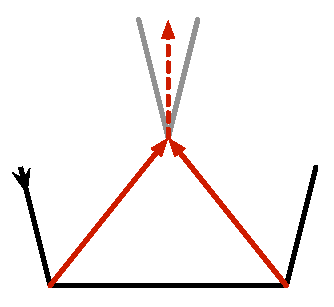
\includegraphics[scale=0.6667]{fig-simple-collapse.pdf}
		\label{fig:simplecollapse}}
\subfigure[Split]{
		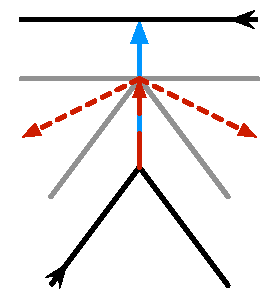
\includegraphics[scale=0.6667]{fig-simple-split.pdf}
		\label{fig:simplesplit}}
\caption{Simple Events.}
\label{fig:simpleevents}
\end{center}
\end{figure}

Simple events, such as in \cref{fig:simpleevents}, are no problem to compute. There is no ambiguity or race condition.


\subsubsection{Simple Degenerate Cases}

\begin{figure}[htpb]
\begin{center}
\subfigure[Simultaneous Collapse]{
		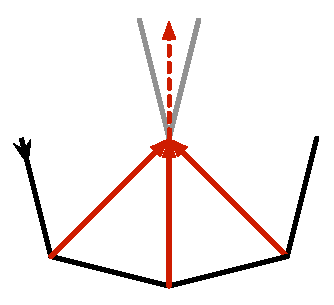
\includegraphics[scale=0.6667]{fig-degenerate-collapse.pdf}
		\label{fig:degeneratecollapse}}
\subfigure[Parallel Neighbours]{
		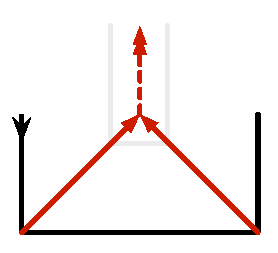
\includegraphics[scale=0.6667]{fig-parallel-collapse.pdf}
		\label{fig:parallelcollapse}}
\subfigure[Parallel Neighbours Reverse]{
		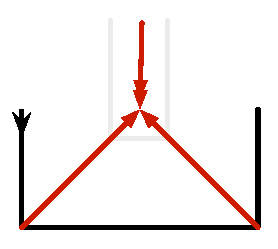
\includegraphics[scale=0.6667]{fig-parallel-collapse2.pdf}
		\label{fig:parallelcollapse2}}
\subfigure[Degenerate Parallel Collapse]{
		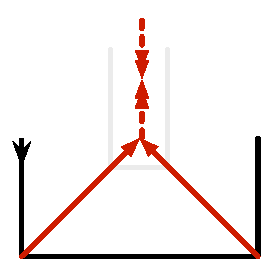
\includegraphics[scale=0.6667]{fig-parallel-collapse3.pdf}
		\label{fig:parallelcollapse3}}
\caption{Degnerate Events.}
\label{fig:degenerateevents}
\end{center}
\end{figure}


Next up are degenerate events. \Cref{fig:degeneratecollapse} shows a form where multiple wavefronts collapse simultaneously in a single point. This kind of event poses no problem, however, as the order of event resolution does not matter. Similarly, \cref{fig:parallelcollapse} is not a problem in itself. The collapse generates a new spoke with infinite velocity. It's reverse condition in  \cref{fig:parallelcollapse2} results in the same situation as \cref{fig:degeneratecollapse}, only that the wavefront propagation terminates. A problem can occur, when the situation in \cref{fig:parallelcollapse3} arises. If the collapses were computed with perfect accuracy, this would be the actual situation, not the two previous cases. Mathematically the two spokes would collide. However, they clearly do have to collide.

The question arises, how a fast\footnote{an angular bisector with infinite speed} spoke should be handled. The fundamental question is, are fast spokes always generated in pairs? If that is the case, the condition can be detected easily, as the two involved wavefronts form a two-member loop.

\subsubsection{Compound Split and Collapse}

\label{sec:compoundsplit}

\begin{figure}[htpb]
\begin{center}
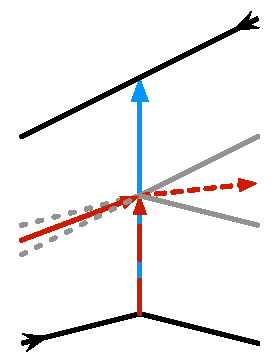
\includegraphics[scale=0.6667]{fig-compound-split-collapse.pdf}
\caption{Compound Split and Collapse.}
\label{fig:compoundcollapse}
\end{center}
\end{figure}


There exist configurations, such as in \cref{fig:compoundcollapse}, which pose timing problems between split and collapse events. In the figure, the left side of the split collapses simultaneously. Due to limited numeric precision, the split or collapse might occur first. If the collapse occurs first, the split should be annulled, and the collapse resolves to the right configuration.

\subsubsection{Terminal Split}

\begin{figure}[htpb]
\begin{center}
\subfigure[Terminal Split Theory]{
		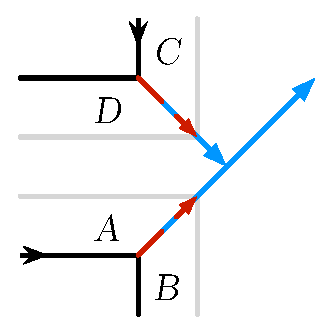
\includegraphics[scale=0.6667]{fig-terminal-split.pdf}
		\label{fig:terminalsplit:theory}}
\subfigure[Terminal Split Ideal]{
		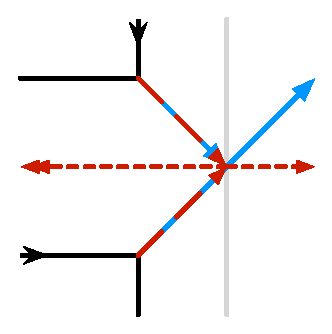
\includegraphics[scale=0.6667]{fig-terminal-split-ideal.pdf}
		\label{fig:terminalsplit:ideal}}
\subfigure[Terminal Split Actual]{
		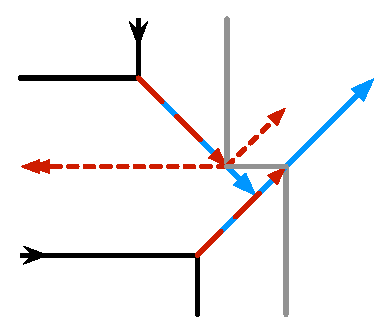
\includegraphics[scale=0.6667]{fig-terminal-split2.pdf}
		\label{fig:terminalsplit:actual}}
\caption{Terminal Split Edge Case.}
\label{fig:terminalsplit}
\end{center}
\end{figure}


\Cref{fig:terminalsplit:theory} poses another challenge. Intuitively, the split should occur so that \cref{fig:terminalsplit:ideal} is the result. However, the wavefront graph is such that bisector $CD$ will split wavefront $A$, thus resulting in a situation as in \cref{fig:terminalsplit:actual}, with a leftover fragment of $A$, potentially of infinite length, if $AB$ and $CD$ meet where the split would occur.

If the leftover fragment of $A$ is of finite size, the geometry is not degenerate, though unintuitive. However, an infinitely small wavefront with parallel spokes poses a problem

Some important questions are:

\paragraph{Can the event location be such that wavefronts $C$ and $B$ are oppositely ordered to \cref{fig:terminalsplit:actual}?} This case should not occur, as if $CD$ reaches the meeting point before $AB$, then motorcycle $AB$ would terminate, and the roles of the two motorcycles would be reversed, thus resulting in the same configuration, only mirrored vertically.

The intersection point of $AB,CD$ may be exactly in between grid cells, in which case edges $A,D$ will not be in the same grid cell along $CD$ at any point in time. In this case, the point closer to the origin of $CD$ should be chosen as the split location, as that will always result in a configuration such as \cref{fig:terminalsplit:actual}.

\paragraph{Is a zero-length leftover segment of $A$ a problem in further wave propagation?} This question assumes that the situation is exactly as in \cref{fig:terminalsplit:theory}, with $AB$ and $CD$ reaching their intersection points at exactly the same time.

\begin{figure}[htpb]
\begin{center}
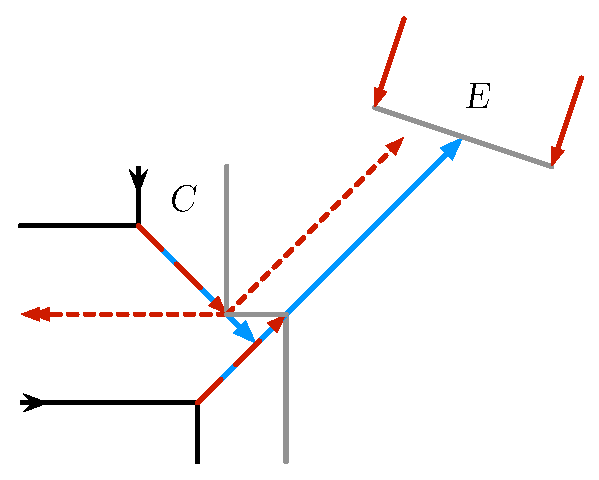
\includegraphics[scale=0.6667]{fig-terminal-split3.pdf}
\caption{Resolution of split following terminal split.}
\label{fig:terminalsplit:order}
\end{center}
\end{figure}

If the split and terminal vertices are exactly coincident, there is a conflict with the situation as laid out in \cref{sec:compoundsplit}. As shown in \cref{fig:terminalsplit:order}, the collapse of wavefront $C$ should normally occur after the edge $E$ is split. If both coincide, however, the condition that a split follows a collapse at a given location and time, must be refined.

In the case of coincidence, it seems reasonable to discard the vestigial wavefront immediately, when evaluating the original split event. Coincidence in this case is defined by exactly coincident virtual source vertices for the two spokes, as well as their colinearity.

 
\subsubsection{Parallel Non-Split}


\begin{figure}[htpb]
\begin{center}
\subfigure[Problem]{
		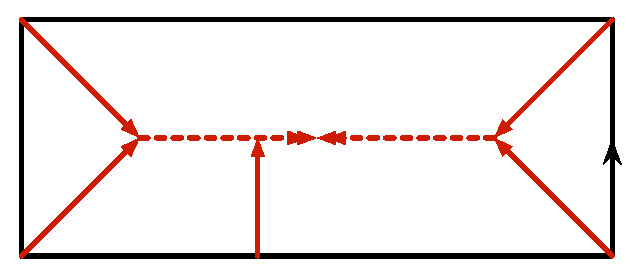
\includegraphics[scale=0.6667]{fig-parallel-non-split.pdf}
		\label{fig:parallelnonsplit:problem}}
\subfigure[Solution]{
		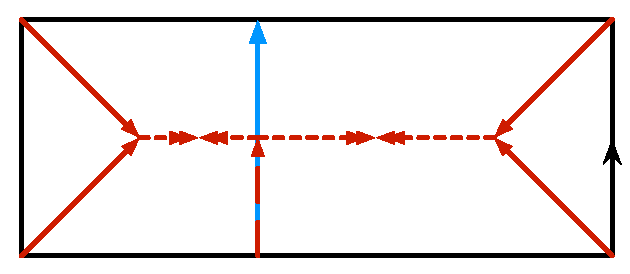
\includegraphics[scale=0.6667]{fig-parallel-non-split-solution.pdf}
		\label{fig:parallelnonsplit:solution}}
\caption{Degenerate Split.}
\label{fig:parallelnonsplit}
\end{center}
\end{figure}


\Cref{fig:parallelnonsplit} depicts a situation in which the bottom edge is made up of two parts which are not strictly concave, but exactly parallel. This case illustrates that a motorcycle must be generated 

\subsubsection{The Degenerate Cross}

\begin{figure}[htpb]
\begin{center}
\subfigure[Ambiguous Cross]{
		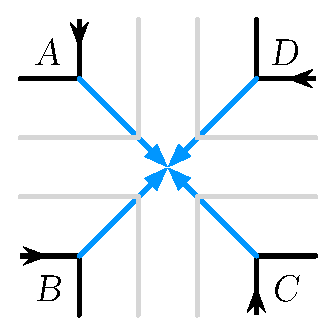
\includegraphics[scale=0.6667]{fig-degenerate-cross.pdf}
		\label{fig:degeneratecross:ambiguity}}
\subfigure[Wheel]{
		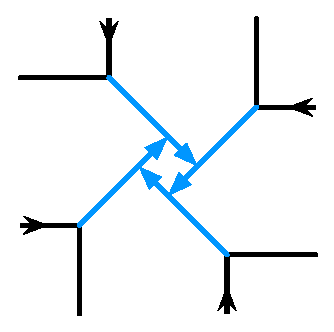
\includegraphics[scale=0.6667]{fig-degenerate-cross2.pdf}
		\label{fig:degeneratecross:wheel}}
\subfigure[Z]{
		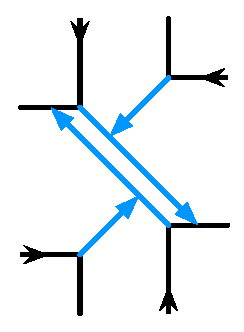
\includegraphics[scale=0.6667]{fig-degenerate-cross3.pdf}
		\label{fig:degeneratecross:z}}
\subfigure[Asymmetric]{
		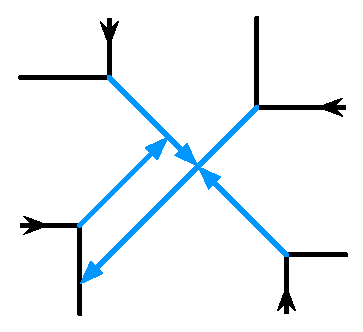
\includegraphics[scale=0.6667]{fig-degenerate-cross4.pdf}
		\label{fig:degeneratecross:asymmetric}}
\caption{Degenerate Cross Motorcycle Graph.}
\label{fig:degeneratecross}
\end{center}
\end{figure}


The degenerate cross configuration shown in \cref{fig:degeneratecross:ambiguity} is already non-deterministic at the motorcycle tracing phase, possibly leading to problems later on. All four motorcycles reach the intersection point at the same time, and several different arrangements, as depicted in \cref{fig:degeneratecross:wheel,fig:degeneratecross:z,,fig:degeneratecross:asymmetric}, can arise, depending on the starting vertex of the source polygon\footnote{that is the assumption, at least}, even without the depicted displacement of the four vertices.

\Cref{fig:degeneratecross:asymmetric} has been observed to pose a problem, with the result that the split between corners $D,A$ (or $C,D$) is not completed right, when the four corners are in perfect alignment.

Observing the arrangement, the configuration of $D$ seems straight forward, with a clear opposing front to the spoke. Following this, $A$ and $C$ may be assigned to either opposing or neighbour wavefronts, but the opposing wavefront for $B$ is tricky. The opposing front of $A$ should be $D$'s right neighbour, and $B$'s opposing front should be $A$'s right neighbour.

However, 

\subsection{Exactness}

All events during polygon offsetting result from angular bisectors, and the intersections of the angular bisectors and the segments of the source polygon.

\subsubsection{Conclusion}

In conclusion, ???.

%$$ S = v3Add(vReverseProject(v0, e1), vReverseProject(v1, e0))$$

%\printnomenclature
\nocite{*}

\bibliographystyle{ieeetr}
\bibliography{machinist}

\end{document}

